\begin{problem}{Антенна}{стандартный ввод}{стандартный вывод}{1 секунда}{512 мегабайт}

Для связи с Землёй членам экспедиции на Марс необходимо собрать антенну. Антенна в разобранном состоянии представляет собой $n$ фрагментов, $i$-й фрагмент представляет собой штангу длиной $s_i$ сантиметров, на которой закреплены $m_i$ перекладин. Каждый фрагмент содержит хотя бы одну перекладину.

У каждой штанги есть начало, в котором расположен штекер, и конец, в котором расположено гнездо. Любые две штанги можно последовательно соединить, присоединив начало одной к концу другой. Для каждой перекладины известно расстояние от начала её штанги в сантиметрах. Для $i$-го фрагмента это расстояние может быть от $0$ до $s_i$, значение 0 означает, что перекладина находится непосредственно в начале штанги, значение $s_i$ "--- что она находится непосредственно в конце штанги. Толщиной перекладин и размерами штекера и гнезда следует пренебречь.

На рисунке показаны три фрагмента антенны из первого примера и отмечены расстояния от начала штанги до перекладины.

\begin{center}
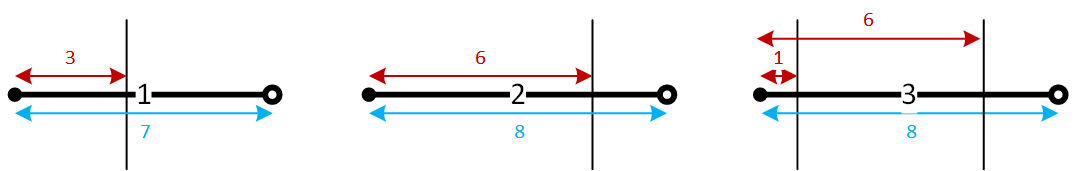
\includegraphics[width=14cm]{parts.png}
\end{center}

Чтобы корректно собрать антенну, необходимо соединить в некотором порядке все $n$ фрагментов, при этом расстояние между любыми двумя соседними перекладинами должно быть одинаковым. 

На рисунке показан корректный способ соединить фрагменты в первом примере.

\begin{center}
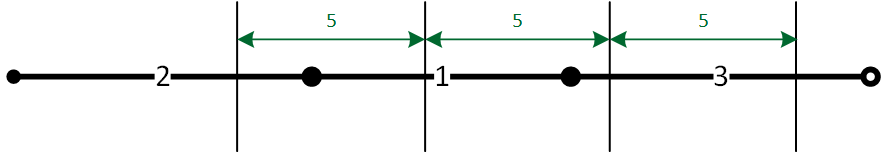
\includegraphics[width=11.53cm]{connected.png}
\end{center}

К сожалению, члены экспедиции забыли инструкцию по сборке антенны на Земле, а передать её на Марс не представляется возможным "--- ведь антенна ещё не собрана. Помогите исследователям!

Требуется определить, в каком порядке необходимо соединить фрагменты антенны, чтобы установить связь с Землей.




\InputFile
В первой строке дано одно число $n$~--- количество фрагментов ($1 \le n \le 100\,000$).

Далее дано описание $n$ фрагментов. В первой строке описания фрагмента даны два целых числа $m_i$ и $s_i$~--- количество перекладин и длина штанги в $i$-м фрагменте ($1 \le m_i \le 100\,000$, $0 \le s_i \le 10^9$). В следующей строке даны $m_i$ целых чисел $p_{i, j}$~--- позиции перекладин, $p_{i, j}$ равно расстоянию в сантиметрах от начала штанги до $j$-й перекладины на ней ($0 \le p_{i, 1} < p_{i, 2} < \dots < p_{i, m_i} \le s_i$).

Сумма всех $m_i$ не превышает $100\,000$.

\OutputFile
Если собрать антенну указанным образом возможно, в первой строке выведите <<\t{Yes}>>, а во второй строке выведите перестановку чисел от $1$ до $n$~--- номера фрагментов в порядке, в котором их следует соединить, начало каждого следующего фрагмента в этом порядке присоединяется к концу предыдущего фрагмента. Если существует несколько подходящих ответов, можно вывести любой из них.

Если собрать антенну невозможно, в единственной строке выведите <<\t{No}>>.


\newpage
\Scoring
Баллы за каждую подзадачу начисляются только в случае, если все тесты для этой
подзадачи и необходимых подзадач успешно пройдены.

\begin{center}
\renewcommand{\arraystretch}{1.3}
\begin{tabular}{|c|c|c|c|c|}
\hline
\textbf{Подзадача} & 
\textbf{Баллы} & 
\textbf{Доп. ограничения} & 
\parbox{3cm}{\textbf{\centering\\Необходимые\\подзадачи\\\vspace{2mm}}} & 
\parbox{3cm}{\textbf{\centering\\Информация\\о проверке\\\vspace{2mm}}} \\
\hline
1 & 8 & $n \le 8$, $m_i = 1$, $s_i \le 100$ & & первая ошибка \\
\hline
2 & 8 & $n \le 8$, $s_i \le 100$ & 1 & первая ошибка \\
\hline
3 & 21 & $n \le 1\,000$ & 1, 2 & первая ошибка \\
\hline
4 & 21 & $\sum m_i > n$ & & первая ошибка \\
\hline
5 & 21 & $s_i \le 100$ & 1, 2 & первая ошибка \\
\hline
6 & 21 & нет & 1--5 & первая ошибка \\
\hline
\end{tabular}
\end{center}

\Examples

\begin{example}
\exmpfile{example.01}{example.01.a}%
\exmpfile{example.02}{example.02.a}%
\exmpfile{example.03}{example.03.a}%
\exmpfile{example.04}{example.04.a}%
\exmpfile{example.05}{example.05.a}%
\end{example}

\end{problem}

